\documentclass[t]{beamer}
\usepackage{hanging}

% Get increased spacing between each item for itemize
\let\tempone\itemize
\let\temptwo\enditemize
\renewenvironment{itemize}{\tempone\addtolength{\itemsep}{0.5\baselineskip}}{\temptwo}

% Get increased spacing between each item for enumerate
\let\tempthree\enumerate
\let\tempfour\endenumerate
\renewenvironment{enumerate}{\tempthree\addtolength{\itemsep}{0.5\baselineskip}}{\tempfour}

\title{Manhattan Rental Market}
\subtitle{Is it as easy as supply and demand?}

\author[W.\,Janson \& D.\,Keller \& S.\,Olalla \& M.\,Wagner]
{%
  \texorpdfstring{
    \begin{columns}%[onlytextwidth]
      \column{.45\linewidth}
      \footnotesize
      \centering
      Wesley Janson\\
      \href{mailto:wrjanson@uchicago.edu}{\texttt{wrjanson@uchicago.edu}}\\
      \vspace*{0.35cm}\\
      Sergio Olalla\\
      \href{mailto:sergiou@uchicago.edu}{\texttt{sergiou@uchicago.edu}}
      \column{.45\linewidth}
      \footnotesize
      \centering
      Drew Keller\\
      \href{mailto:drewkeller@uchicago.edu}{\texttt{drewkeller@uchicago.edu}}\\
      \vspace*{0.35cm}\\
      Michael Wagner\\
      \href{mailto:wagnerm@uchicago.edu}{\texttt{wagnerm@uchicago.edu}}
    \end{columns}
  }
  {Wesley Janson \& Drew Keller \& Sergio Olalla \& Michael Wagner}
}

\institute{\normalsize University of Chicago - MSCA 31006}
\date{March 6, 2023}

\begin{document}

\frame{\titlepage}

\begin{frame}
\frametitle{Introduction}
\begin{itemize}
\item The onset of COVID-19 led to a pronounced urban flight, especially in New York City - the largest rental market in the United States (Whitaker, 2021; Coven et al., 2022)
\item This rapid shift precipitated ``COVID discounts'' on rent...
\item ... followed by a rebound period of returning residents and swift increase in rents
\item We explore COVID's intertwined effects on NYC rent and rental inventory

\end{itemize}
\end{frame}

\begin{frame}
\frametitle{Data}
\begin{itemize}
\item Data from StreetEasy, a NYC Zillow subsidiary
\item StreetEasy publishes monthly series for a number of sale and rental indicators based on its thousands of listings
\item To narrow scope, we specifically look at Manhattan monthly median asking rent and rental inventory
\item We use January 2010 - January 2020 as training data and in a cross-validation approach to assess in-sample model performance
\item We also estimate the effect of COVID in the February 2020 - December 2022 period %\footnote{\tiny{We address how to navigate the COVID-19 period in later slides.}}.

\end{itemize}
\end{frame}

\begin{frame}
\frametitle{Median Rent Data}
\begin{figure}
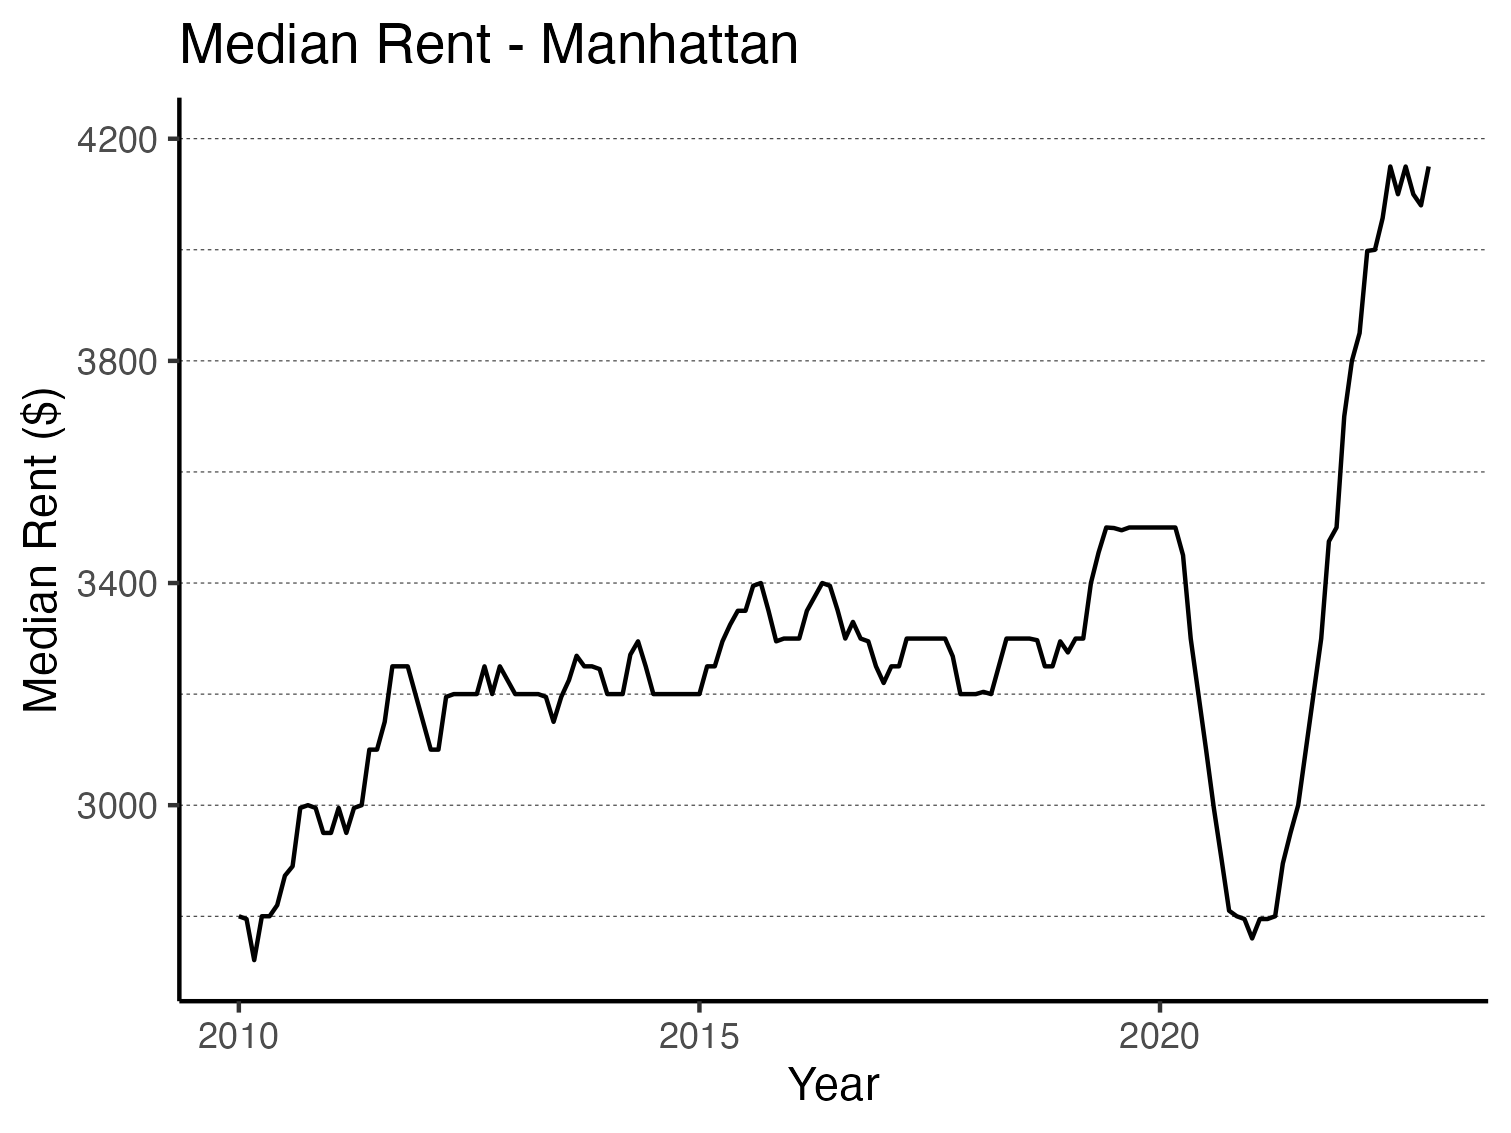
\includegraphics[width=4.2in]{rent_raw_series.png}
\end{figure}
\end{frame}

\begin{frame}
\frametitle{Box-Cox Transformed Median Rent}
\begin{figure}
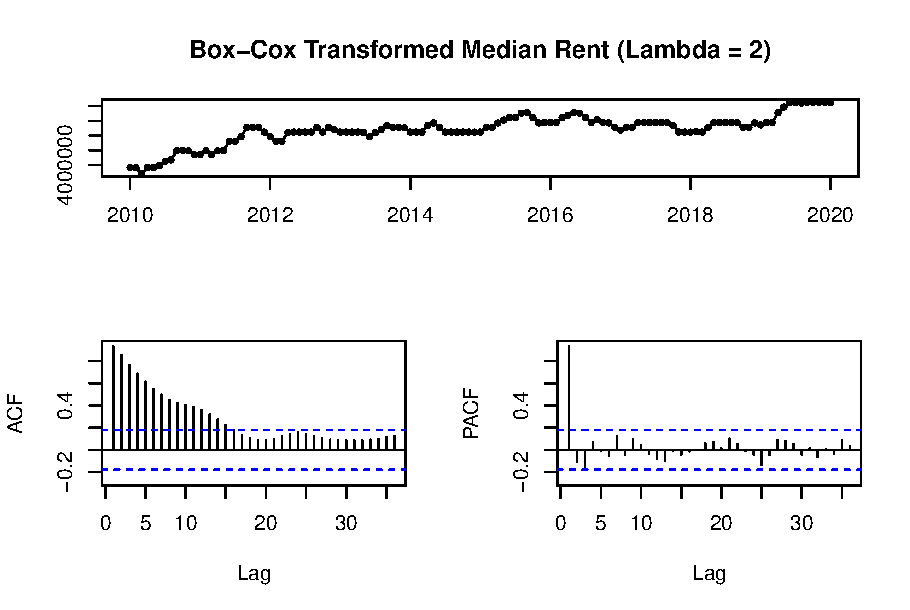
\includegraphics[width=4.2in]{box_cox_rent.pdf}
\end{figure}
\end{frame}

\begin{frame}
\frametitle{Models}
We fit 4 different models:

\begin{enumerate}
\item Seasonal Exponential Smoothing (ETS)
\item Seasonal Autoregressive Integrated Moving Average (sARIMA)
\item Vector Autoregression (VAR)
\item Regression with ARMA errors
\end{enumerate}
\\~\\ %Skip single line
\begin{itemize}
\item Each model is evaluated on in-sample performance and COVID-period analysis
\item Seasonality is annual for all models
\end{itemize}

\end{frame}

\begin{frame}
\frametitle{Exponential Smoothing and sARIMA}
\begin{itemize}
\item Minimum-AICc ETS model is damped additive, and dominated by error term: AAA with $\alpha\approx 1$, $\beta\approx\gamma\approx2*10^{-4}$, $\phi=0.97$
\item Minimum-AICc model is $ARIMA(0,1,0),(2,0,0)_{12}$: nonseasonal component is just first difference, while seasonal component is $AR(2)$; no drift needed
\item Both approaches produce white noise residuals as verified by Ljung-Box test
\end{itemize}
\end{frame}

\begin{frame}
\frametitle{Rent Counterfactual (ETS)}
\begin{figure}
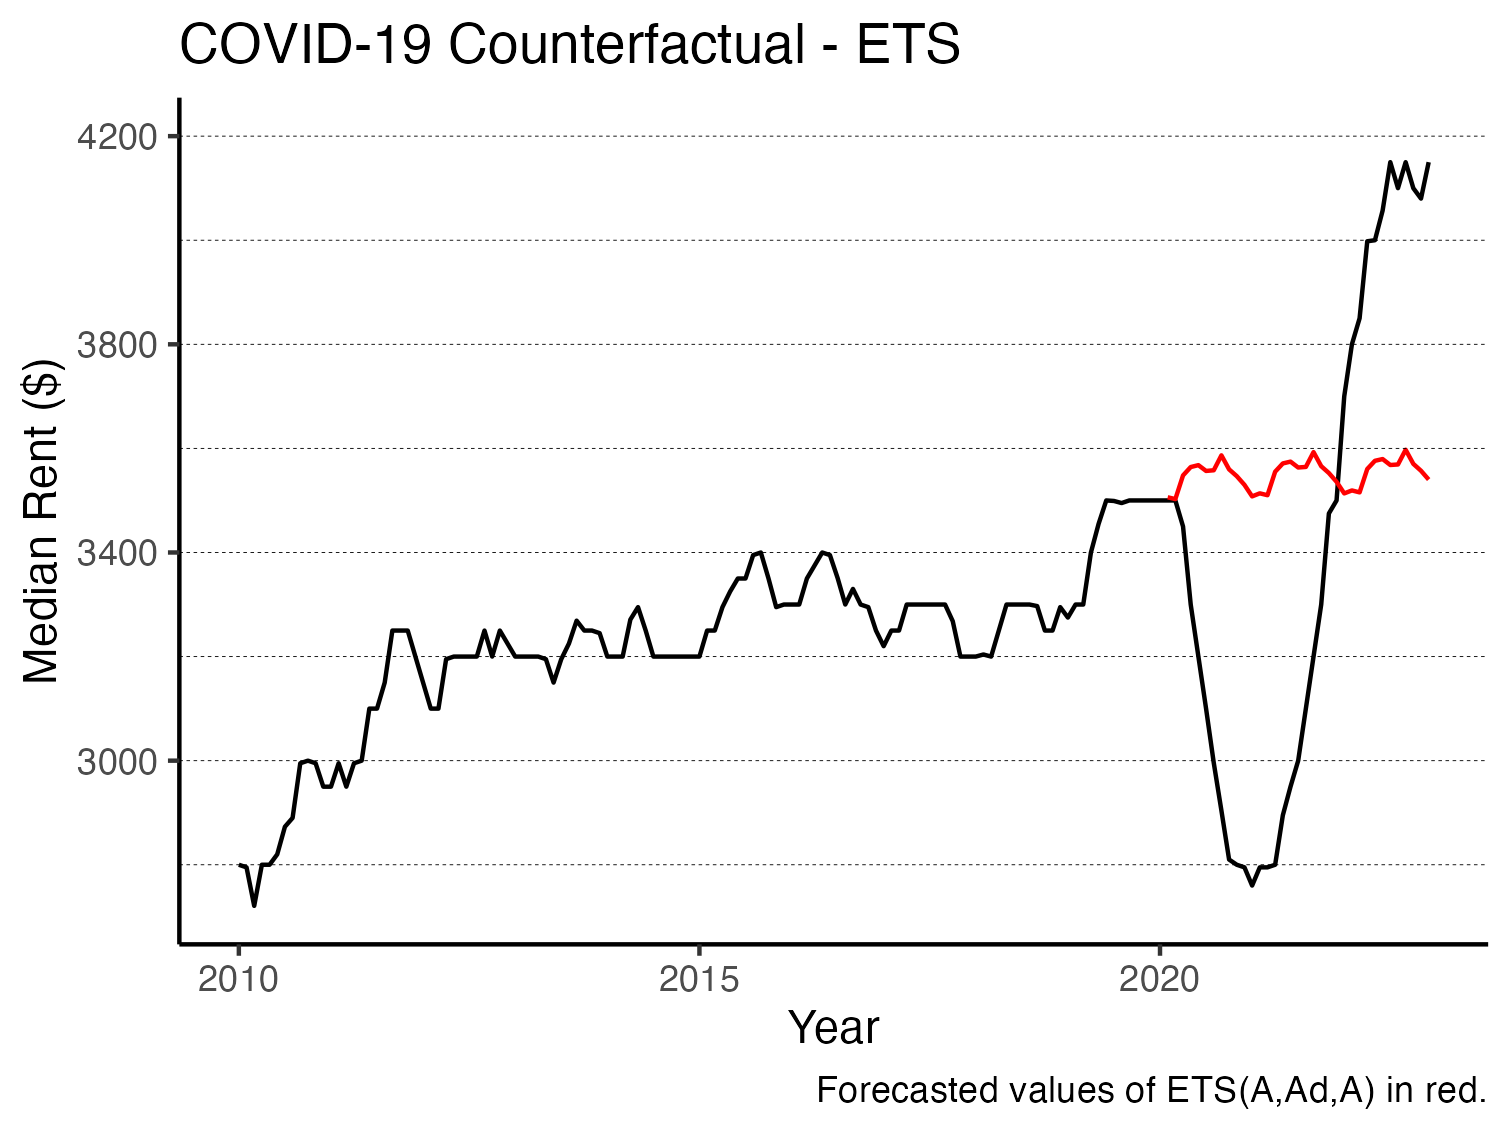
\includegraphics[width= 4.2 in]{rent_counterfactual_ets.png}
\end{figure}
\end{frame}

\begin{frame}
\frametitle{Effect of COVID on Rent}
\begin{figure}
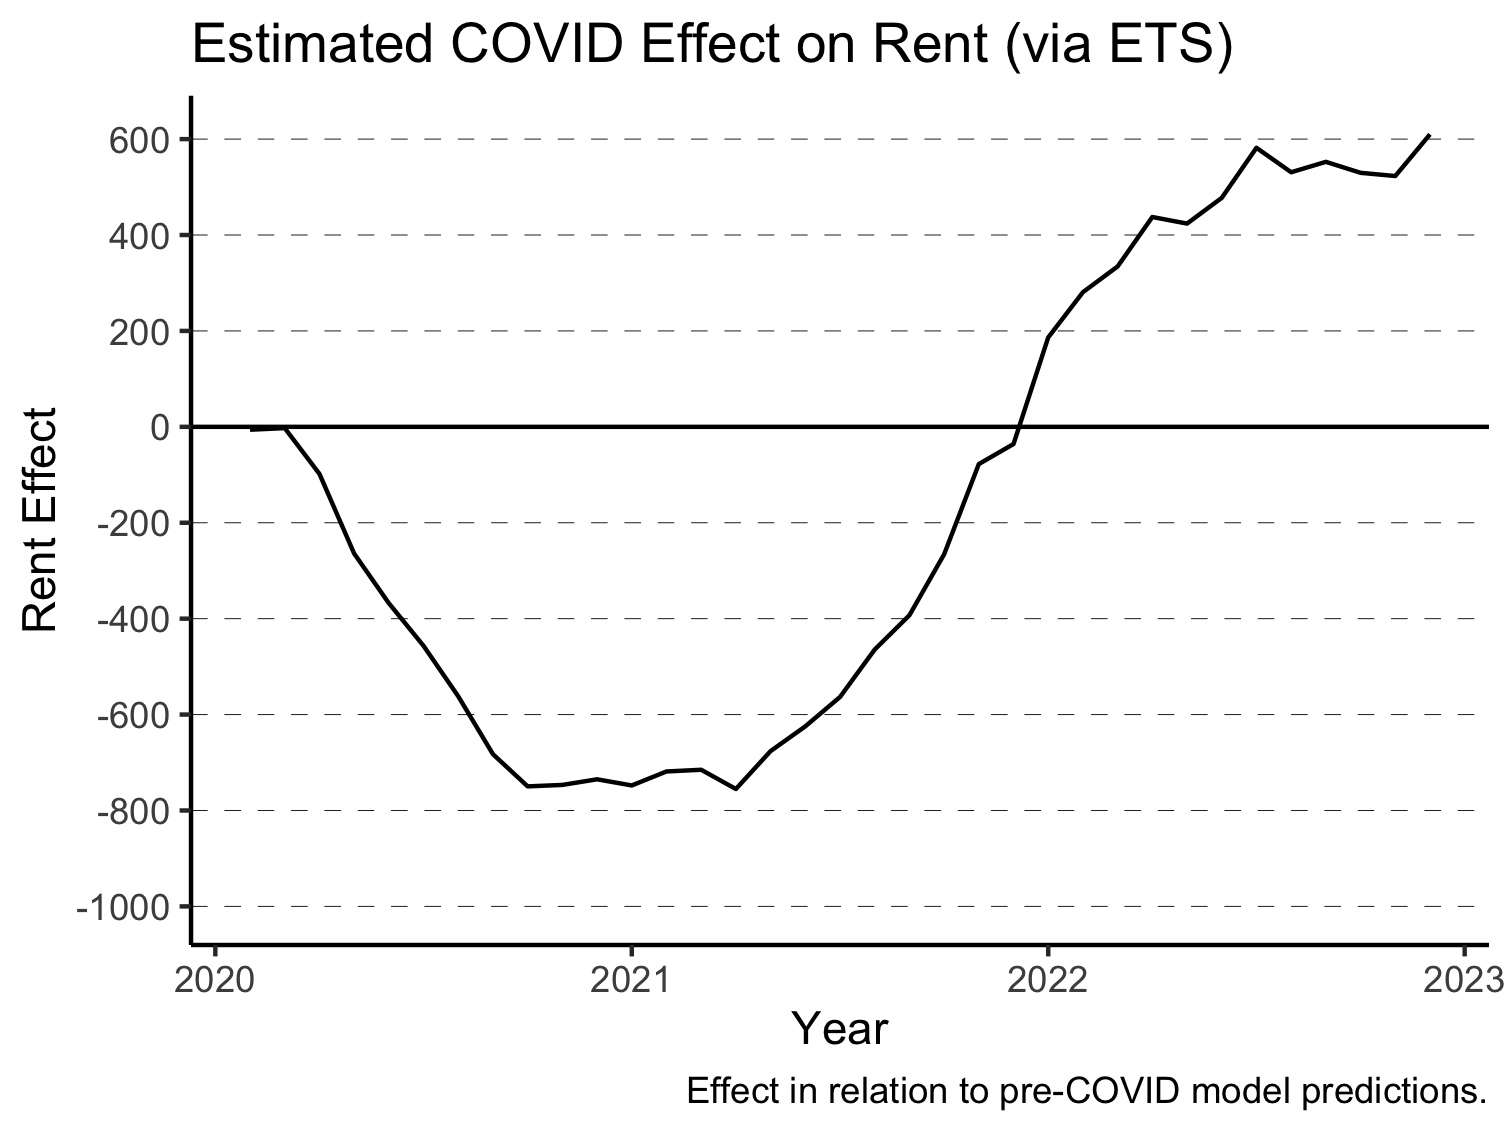
\includegraphics[width= 4.2 in]{rent_covid_effect_ets.png}
\end{figure}
\end{frame}

\begin{frame}
\frametitle{Listing Inventory Data}
\begin{figure}
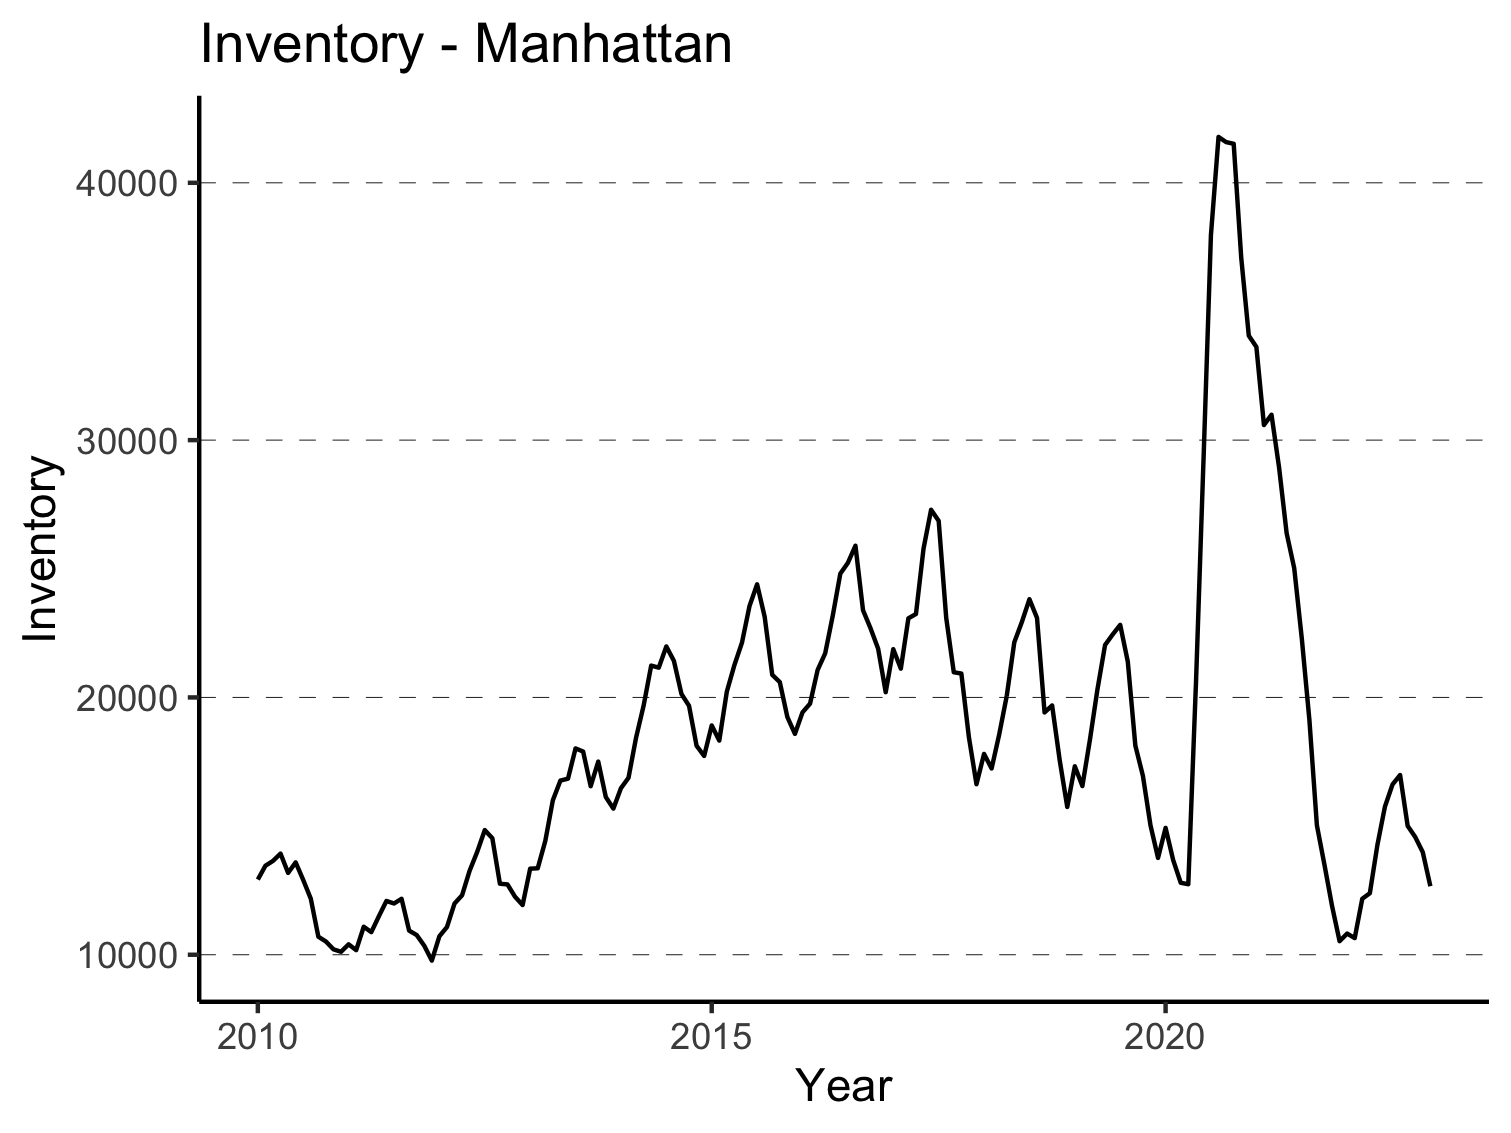
\includegraphics[width=4.2in]{inventory_raw_series.png}
\end{figure}
\end{frame}

\begin{frame}
\frametitle{Box-Cox Transformed Listing Inventory}
\begin{figure}
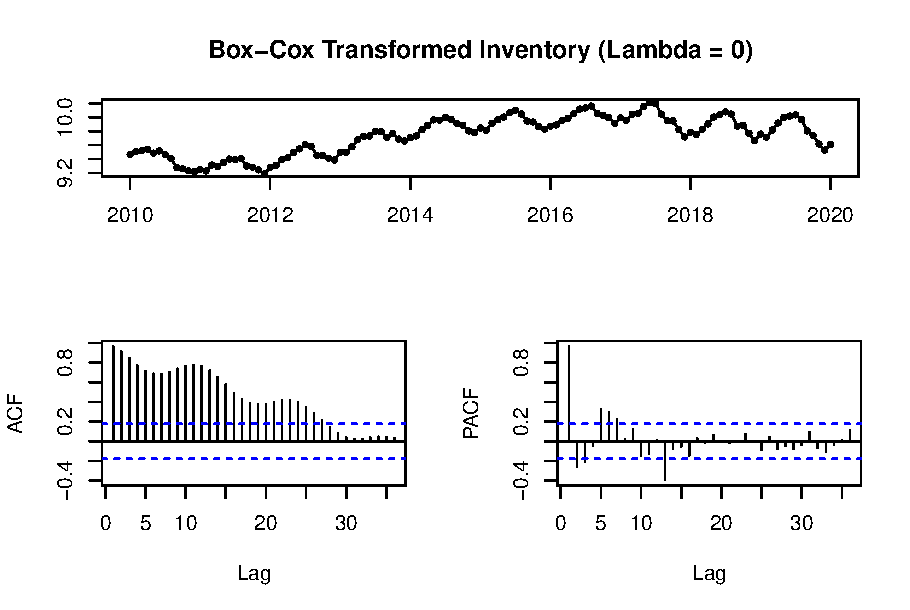
\includegraphics[width=4.2in]{box_cox_inventory.pdf}
\end{figure}
\end{frame}

\begin{frame}
\frametitle{VAR}
\begin{itemize}
\item We test the hypothesis that listing inventory and rent are \textbf{endogenous} with a $VAR(5)$ model
\item Surprisingly, there is largely no significant predictive relationship between the two
\item Select lags of inventory are significant in median rent, but not lags of rent are significant in inventory
\item Though intervention analysis is more complex in the multivariable case, this provides us with a ``COVID counterfactual''\textemdash\text{ }what if COVID-19 never happened?

\end{itemize}
\end{frame}

\begin{frame}
\frametitle{Rent Counterfactual (VAR)}
\begin{figure}
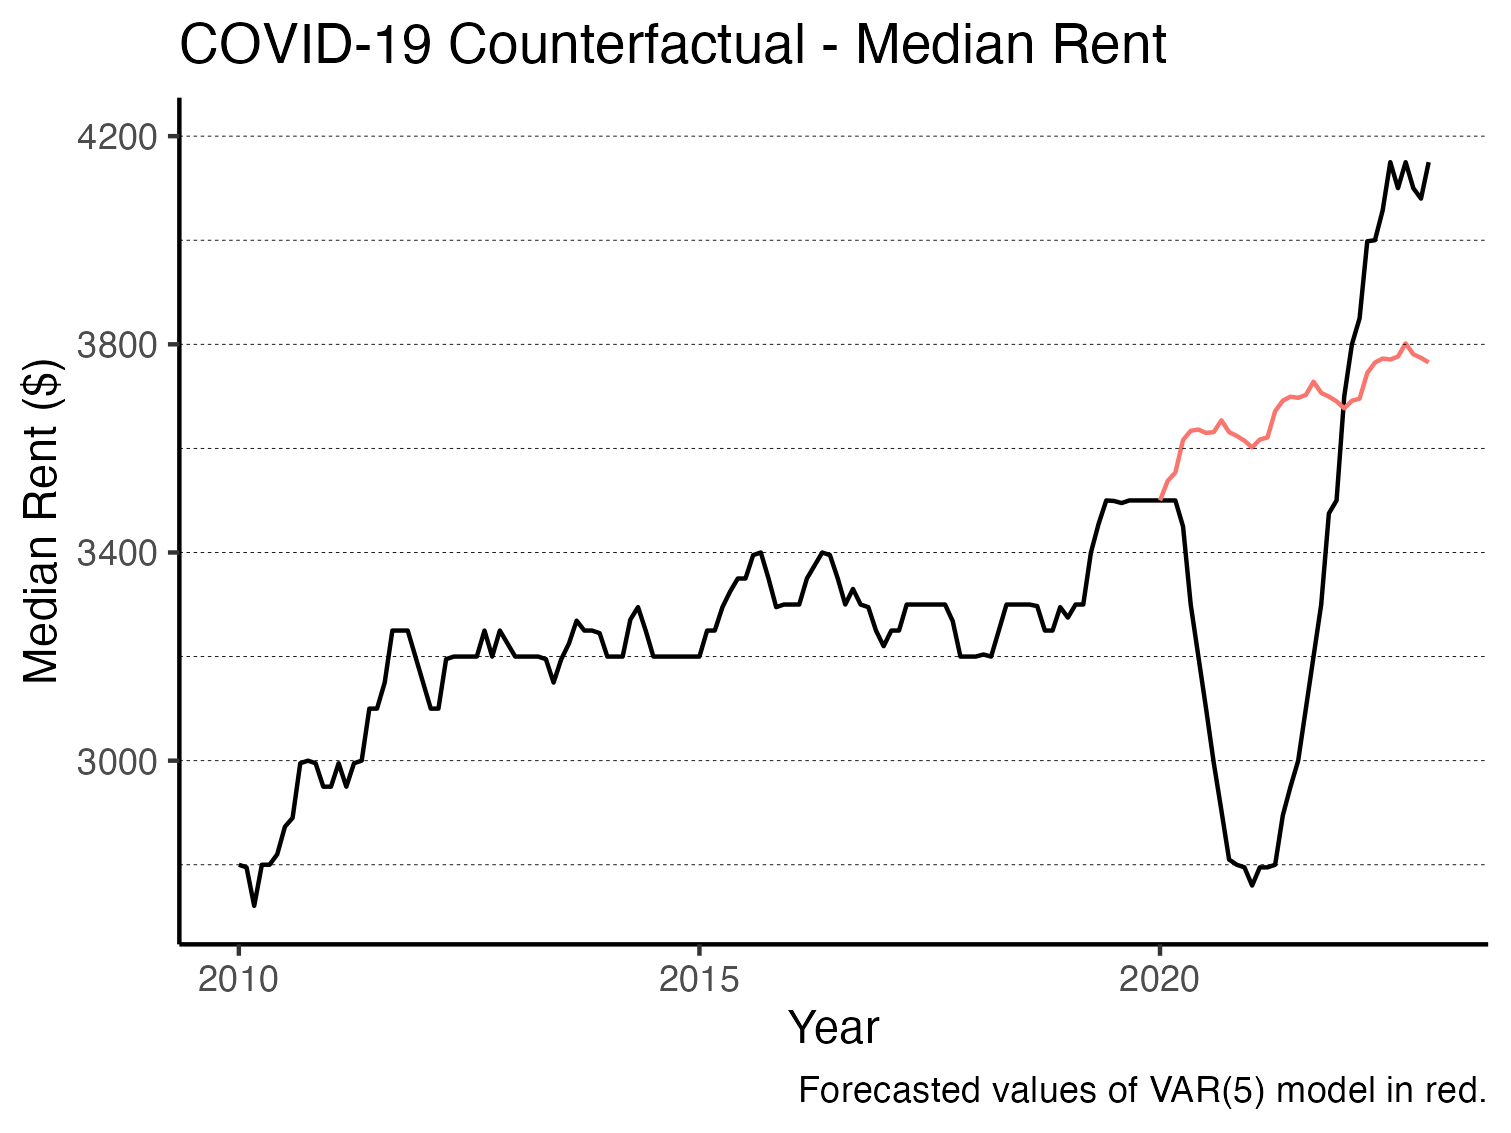
\includegraphics[width=4.2in]{rent_counterfactual.png}
\end{figure}
\end{frame}

\begin{frame}
\frametitle{Regression with ARIMA Errors}
\begin{itemize}
\item Interpretable way to factor in the relationship of an independent variable
\item OLS estimation, while allowing for standard errors to follow ARIMA process
\item Using listing inventory as a covariate, but now determined \textbf{\emph{exogenously}}
\item Inventory forecasted using $ARIMA(0,1,0)(0,1,1)_{12}$ with $\lambda=0$

\end{itemize}
\end{frame}

\begin{frame}
\frametitle{Rent Counterfactual (Regression w/ ARIMA Errors)}
\begin{figure}
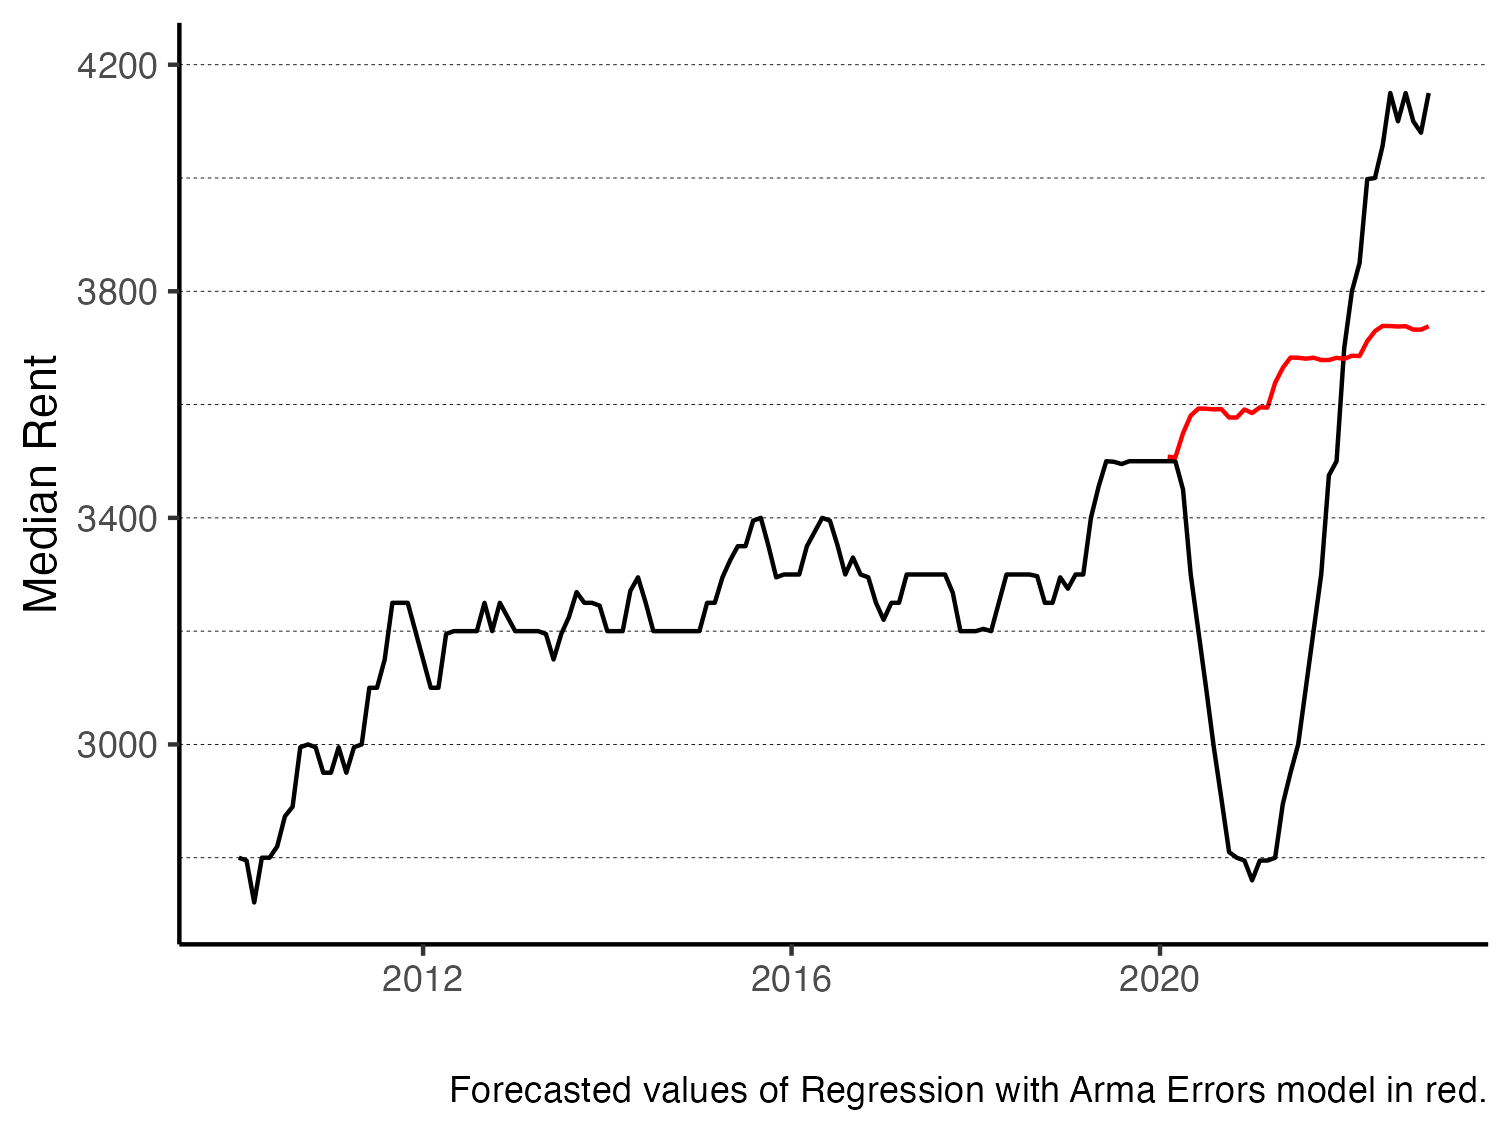
\includegraphics[width= 4.2 in]{rent_counterfactual_arma_error.png}
\end{figure}
\end{frame}

\begin{frame}
\frametitle{In-Sample Cross-Validation on Median Rent}
\begin{figure}
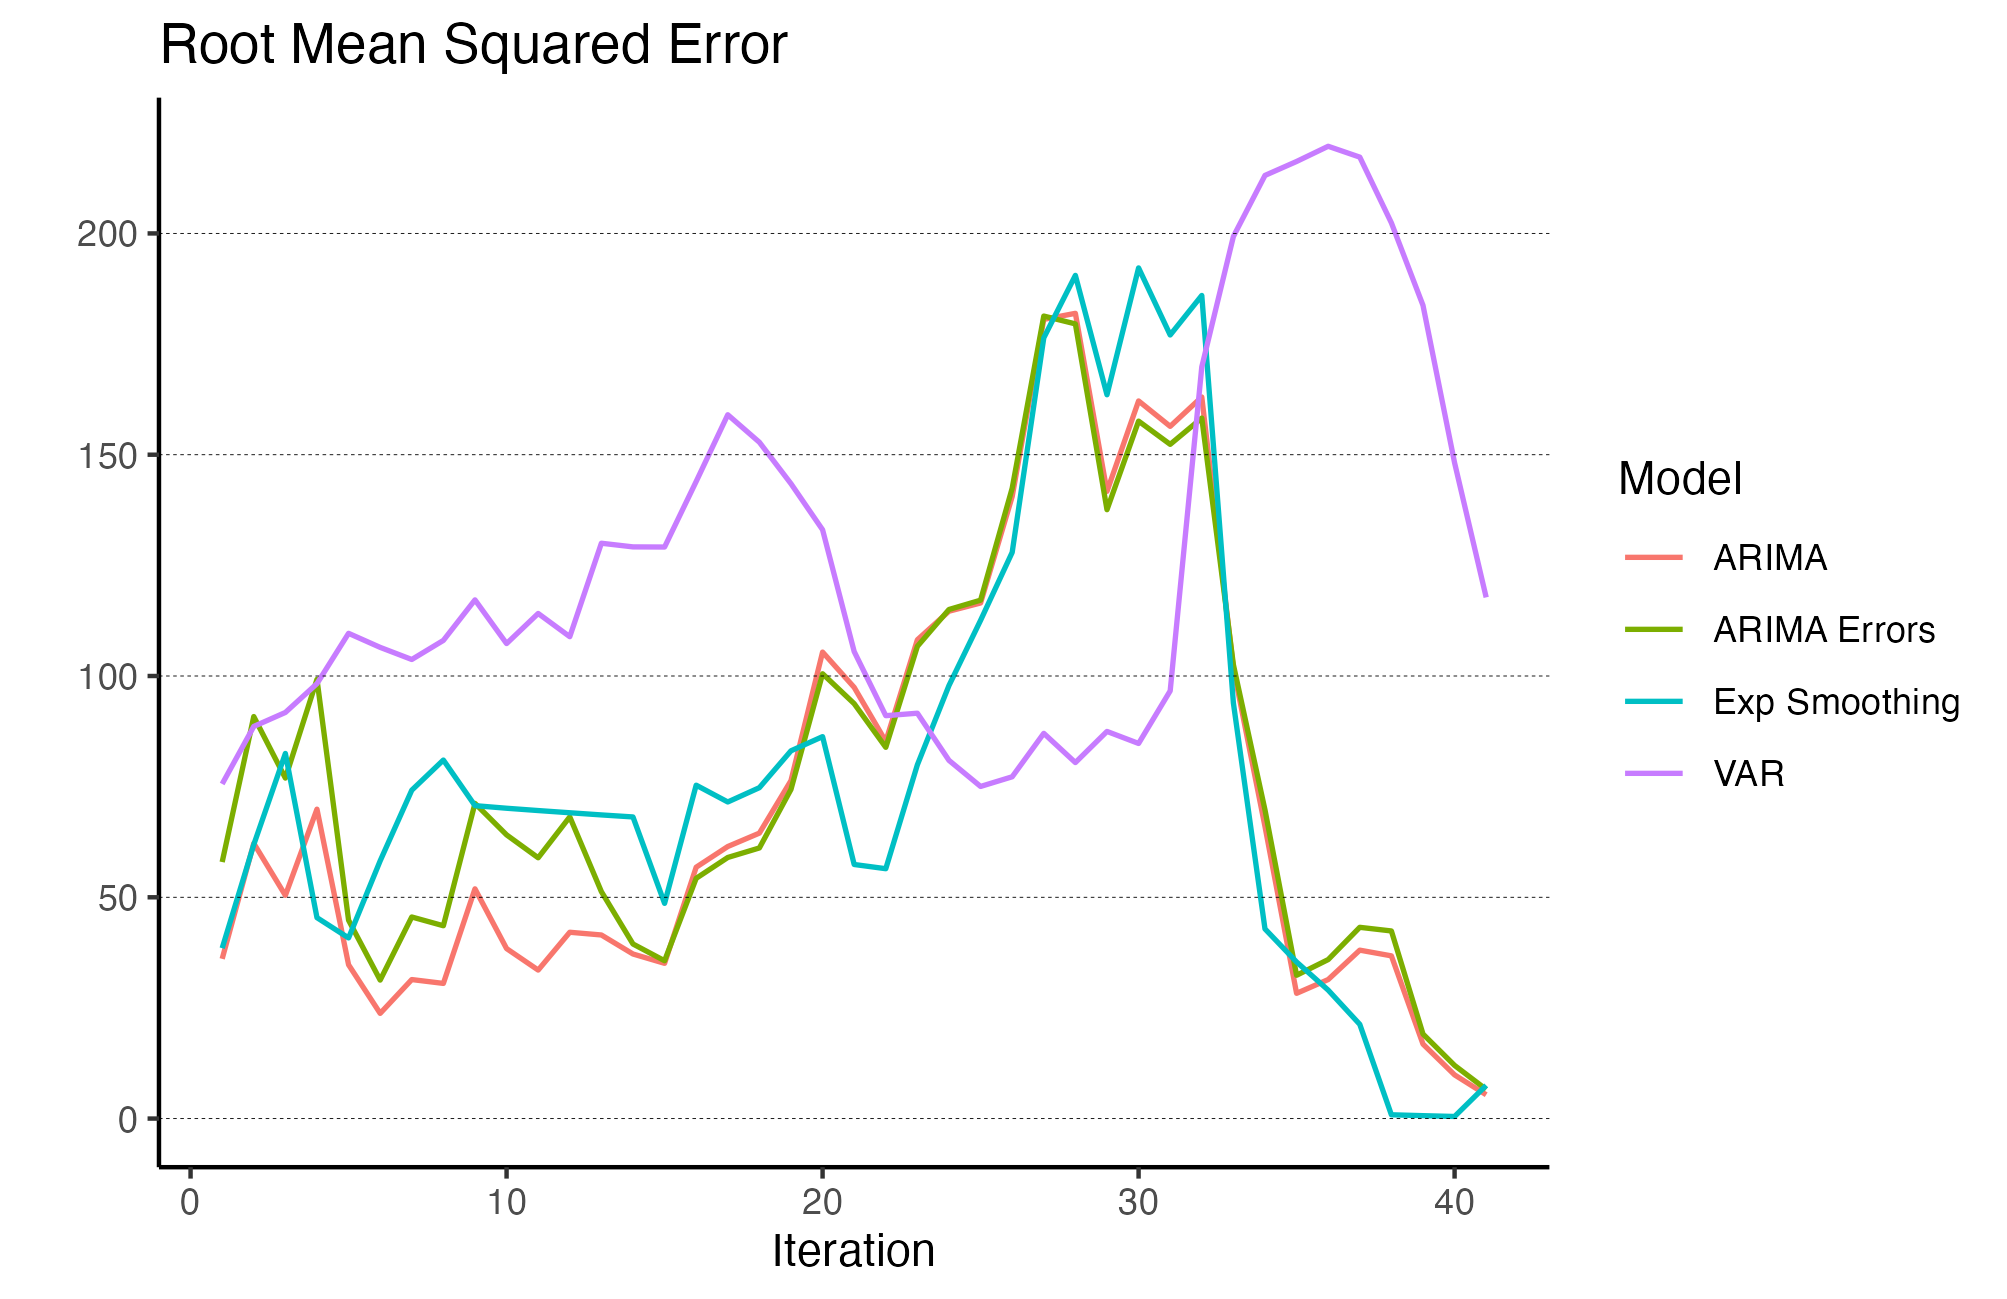
\includegraphics[width=4.5in]{final_cv_results_graph.png}
\end{figure}
\end{frame}

\begin{frame}
\frametitle{Conclusion}
\begin{itemize}
\item Multiple basic approaches produce solid, fairly equivalent models of Manhattan rent in the pre-COVID period
\item COVID's onset marked a major departure from stationarity; intervention analysis methods show it has had a lasting impact on rent (despite a return to baseline of rental inventory)
\item Rental inventory has limited use as a predictor of future rents, but not vice versa
\end{itemize}
\end{frame}

\begin{frame}
\frametitle{Future Work}

\begin{itemize}
\item Continued impact of COVID: With more time will rent slowly return to ``steady state'' level and trend?

\item Would data from a more comprehensive sample of rental units yield different results? Does StreetEasy have an upward/downward bias in rental price or inventory?

\item What is the interaction between rents (and inventory) in different neighborhoods, or even different cities? Can we estimate spillover effects?

\item Is inventory too aggregated of a variable? It represents equilibrium effects\textemdash would showing more demand/supply side variables of the rental market be more advantageous?
\end{itemize}

\end{frame}

\begin{frame}
\frametitle{References}

\begin{hangparas}{.25in}{1}

Coven, J., Gupta, A., & Yao, I. (2022). JUE Insight: Urban Flight Seeded the COVID-19 Pandemic Across the United States. Journal of Urban Economics, 103489.
\\~\\ %Skip single line
Whitaker, Stephan D. 2021. ``Did the COVID-19 Pandemic Cause an Urban Exodus?'' Federal Reserve Bank of Cleveland, Cleveland Fed District Data Brief . \href{https://www.clevelandfed.org/publications/cleveland-fed-district-data-brief/2021/cfddb-20210205-did-the-covid-19-pandemic-cause-an-urban-exodus}{https://doi.org/10.26509/frbc-ddb-20210205}

\end{hangparas}
\end{frame}

\begin{frame}
\frametitle{}
\Large{\textbf{Appendix}}
\end{frame}

\begin{frame}
\frametitle{Individual Contributions}
\begin{itemize}
\doublespacing
\item Wesley: Quality control on modeling, futile attempt at sVARIMA model, slide creation logistics

\item Drew: Dataset finding, sARIMA and ETS modeling, base cross-validation script

\item Sergio: VAR modeling, slide editing

\item Michael: Regression with ARIMA Errors modeling, slide editing
\end{itemize}
\end{frame}

\begin{frame}
\frametitle{COVID-19 Effect on Median Rent}
\begin{figure}
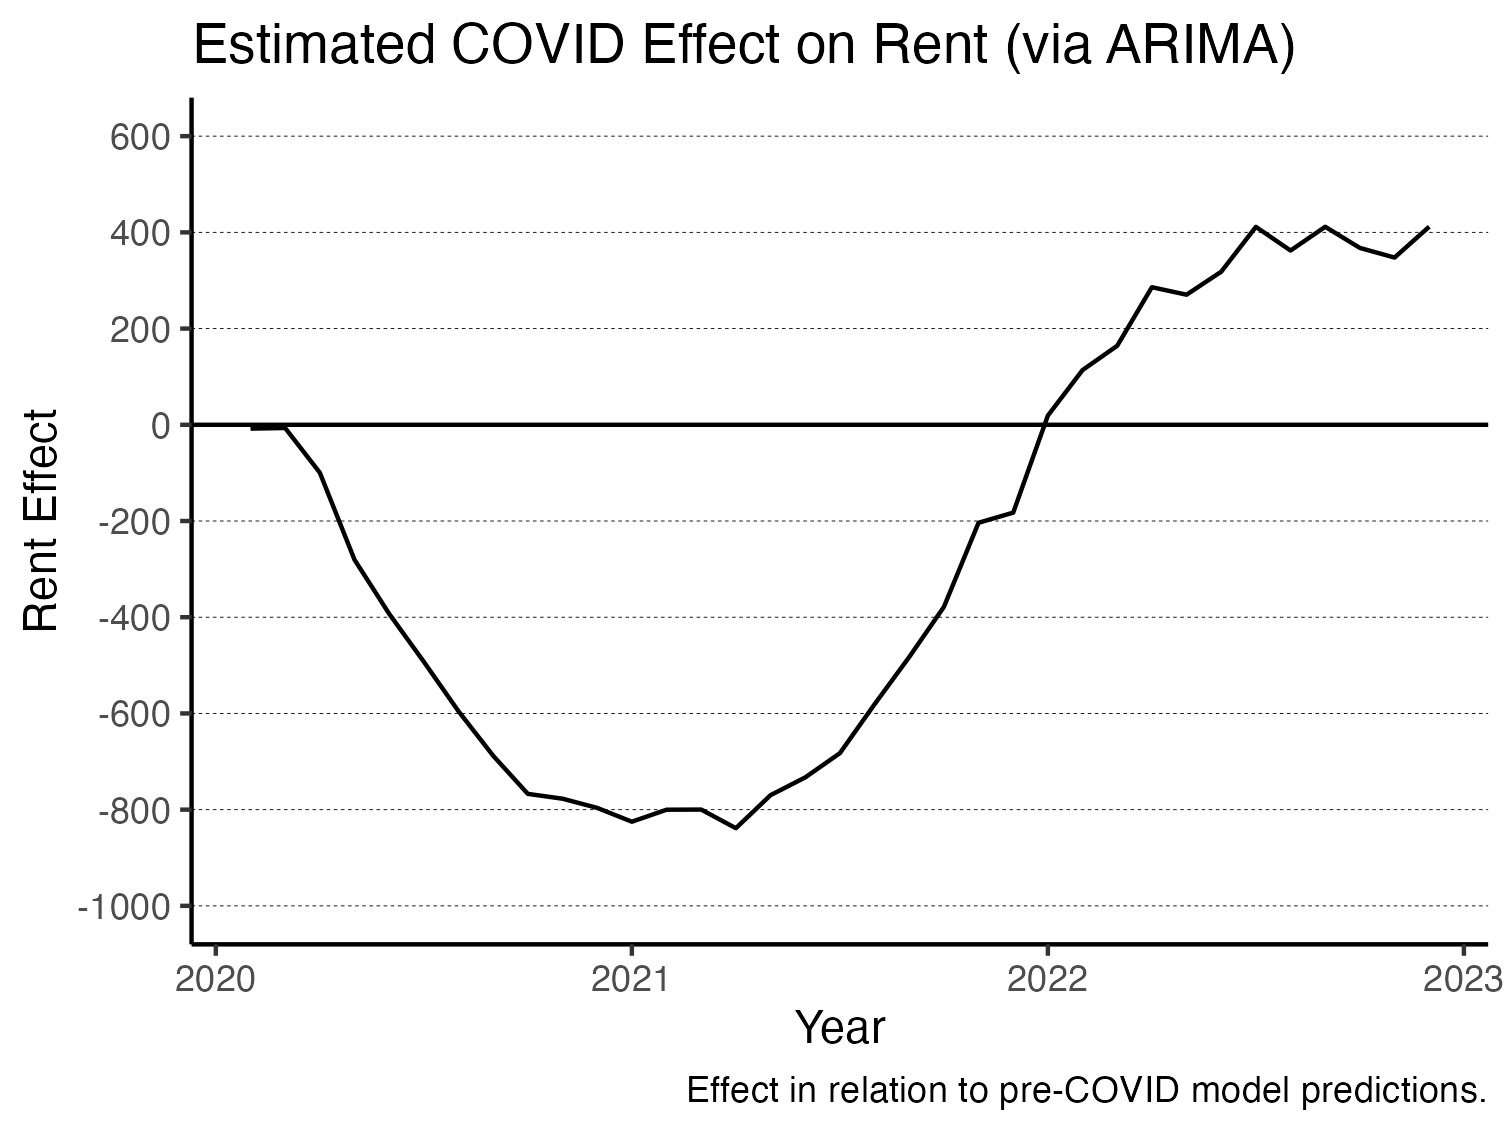
\includegraphics[width=4.2in]{rent_covid_effect.png}
\end{figure}
\end{frame}

\begin{frame}
\frametitle{COVID-19 Effect on Inventory}
\begin{figure}
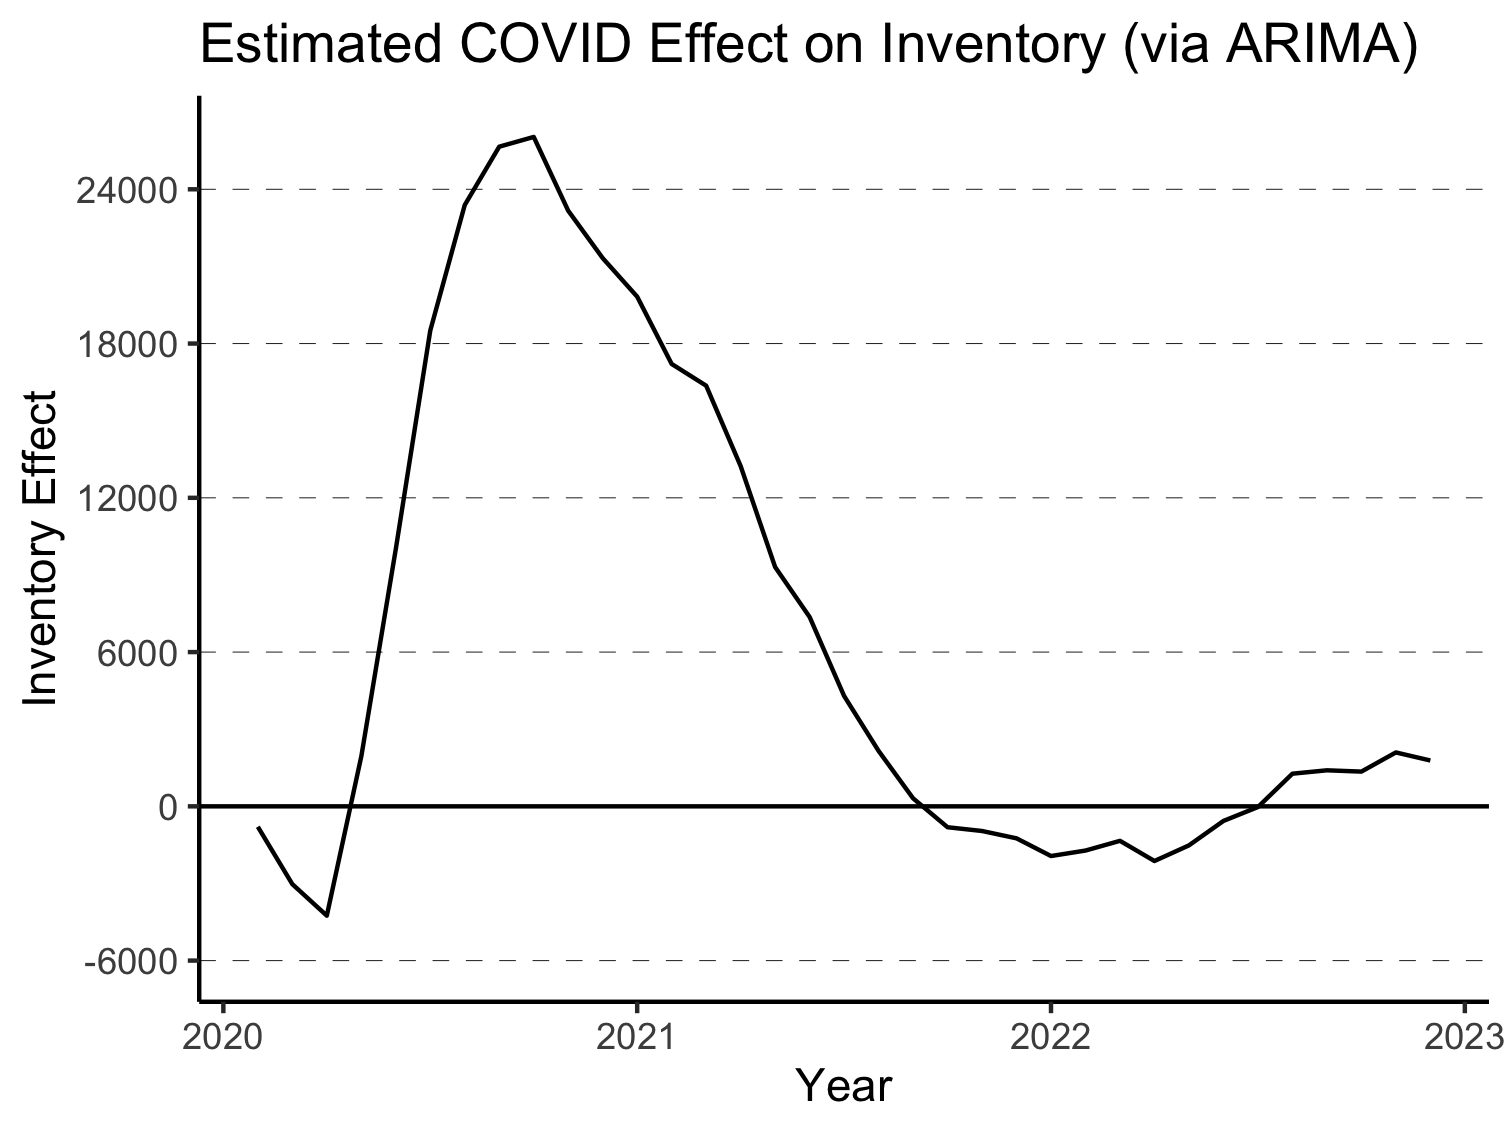
\includegraphics[width=4.2in]{inventory_covid_effect.png}
\end{figure}
\end{frame}

\begin{frame}
\frametitle{Inventory Counterfactual (VAR)}
\begin{figure}
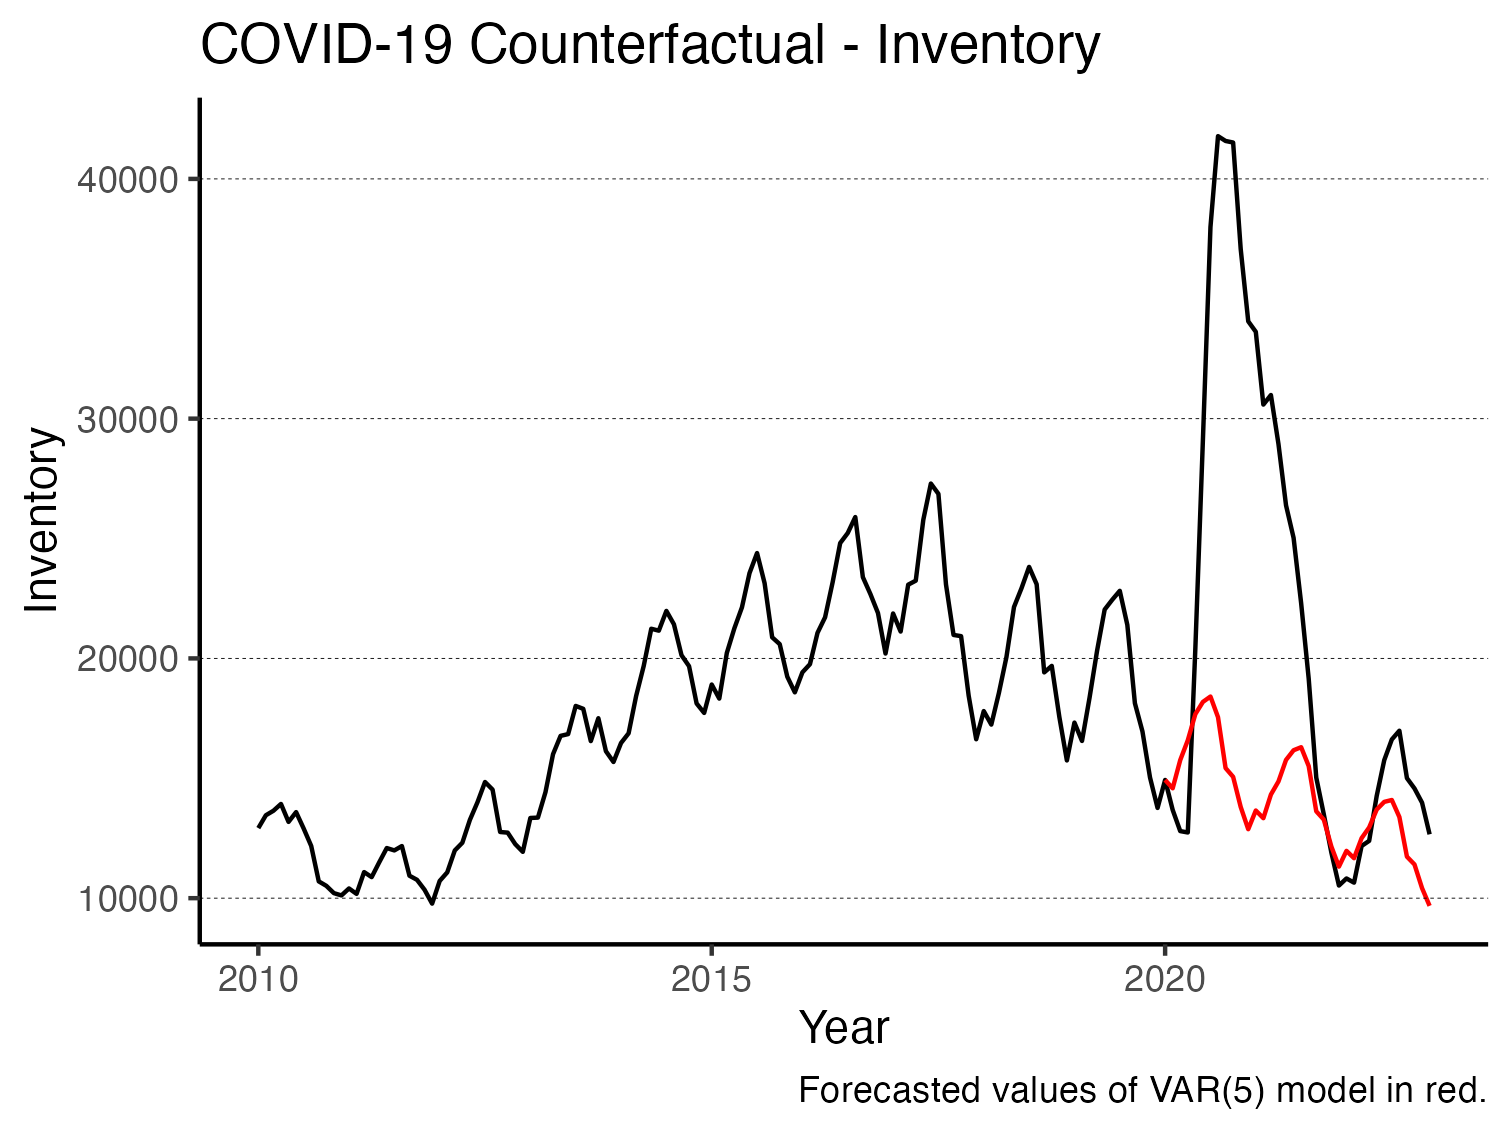
\includegraphics[width=4.2in]{inventory_counterfactual.png}
\end{figure}
\end{frame}

\begin{frame}
\frametitle{ETS Model Residuals (Median Rent)}
\begin{figure}
\includegraphics[width=4.2in]{rent_ets_resid.png}
\end{figure}
\end{frame}

\begin{frame}
\frametitle{ETS Model Residuals (Listing Inventory)}
\begin{figure}
\includegraphics[width=4.2in]{inventory_ets_resid.png}
\end{figure}
\end{frame}

\begin{frame}
\frametitle{sARIMA Model Residuals (Median Rent)}
\begin{figure}
\includegraphics[width=4.2in]{rent_arima_resid.png}
\end{figure}
\end{frame}

\begin{frame}
\frametitle{sARIMA Model Residuals (Listing Inventory)}
\begin{figure}
\includegraphics[width=4.2in]{inventory_arima_resid.png}
\end{figure}
\end{frame}

\begin{frame}
\frametitle{Regression with ARIMA Errors Residuals}
\begin{figure}
\includegraphics[width=4.2in]{residuals_regression_arma_errors.png}
\end{figure}
\end{frame}

\begin{frame}
\frametitle{VAR(5) Model Residuals (Median Rent)}
\begin{figure}
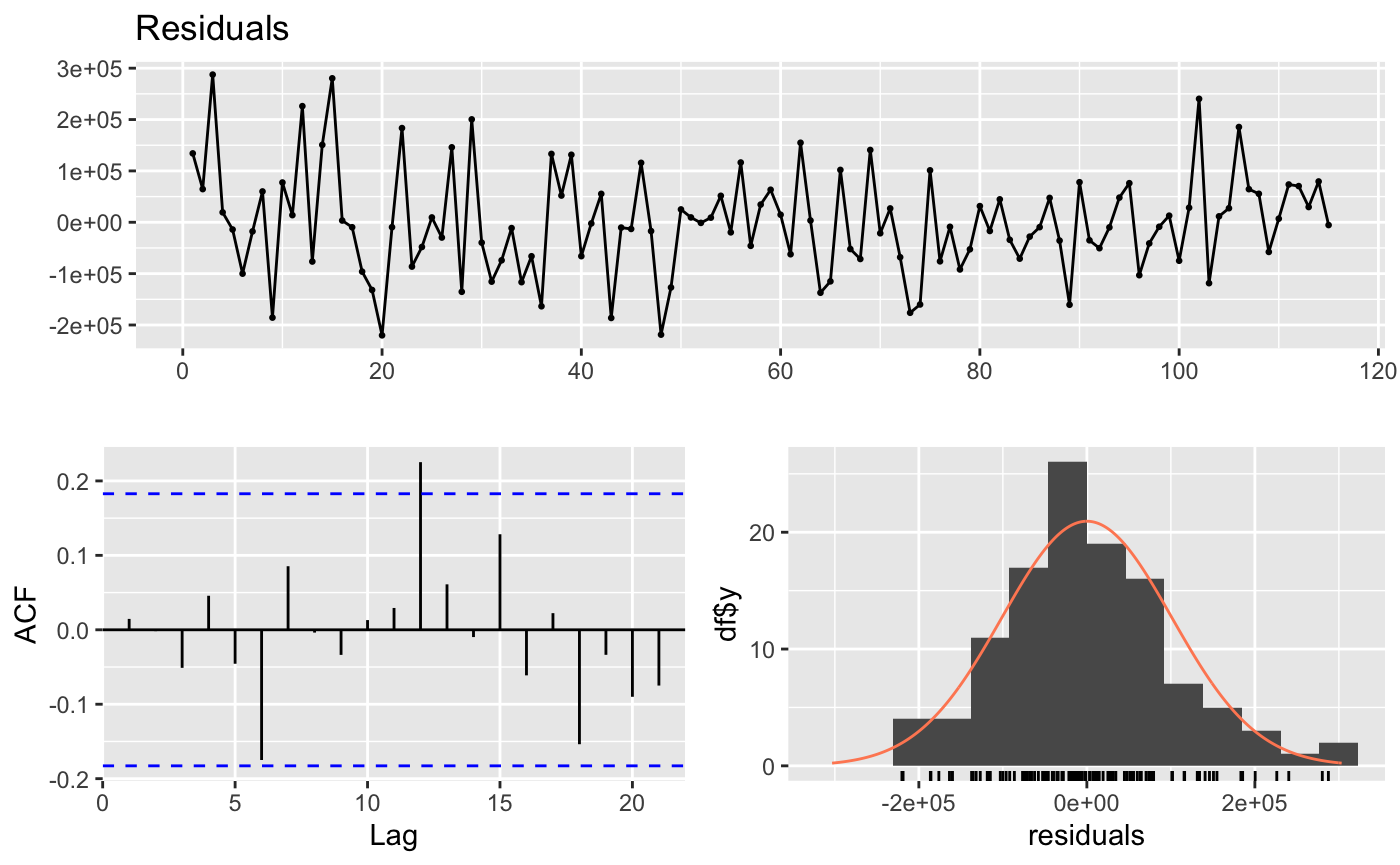
\includegraphics[width=4.2in]{var1_residuals.png}
\end{figure}
\end{frame}

\begin{frame}
\frametitle{VAR(5) Model Residuals (Listing Inventory)}
\begin{figure}
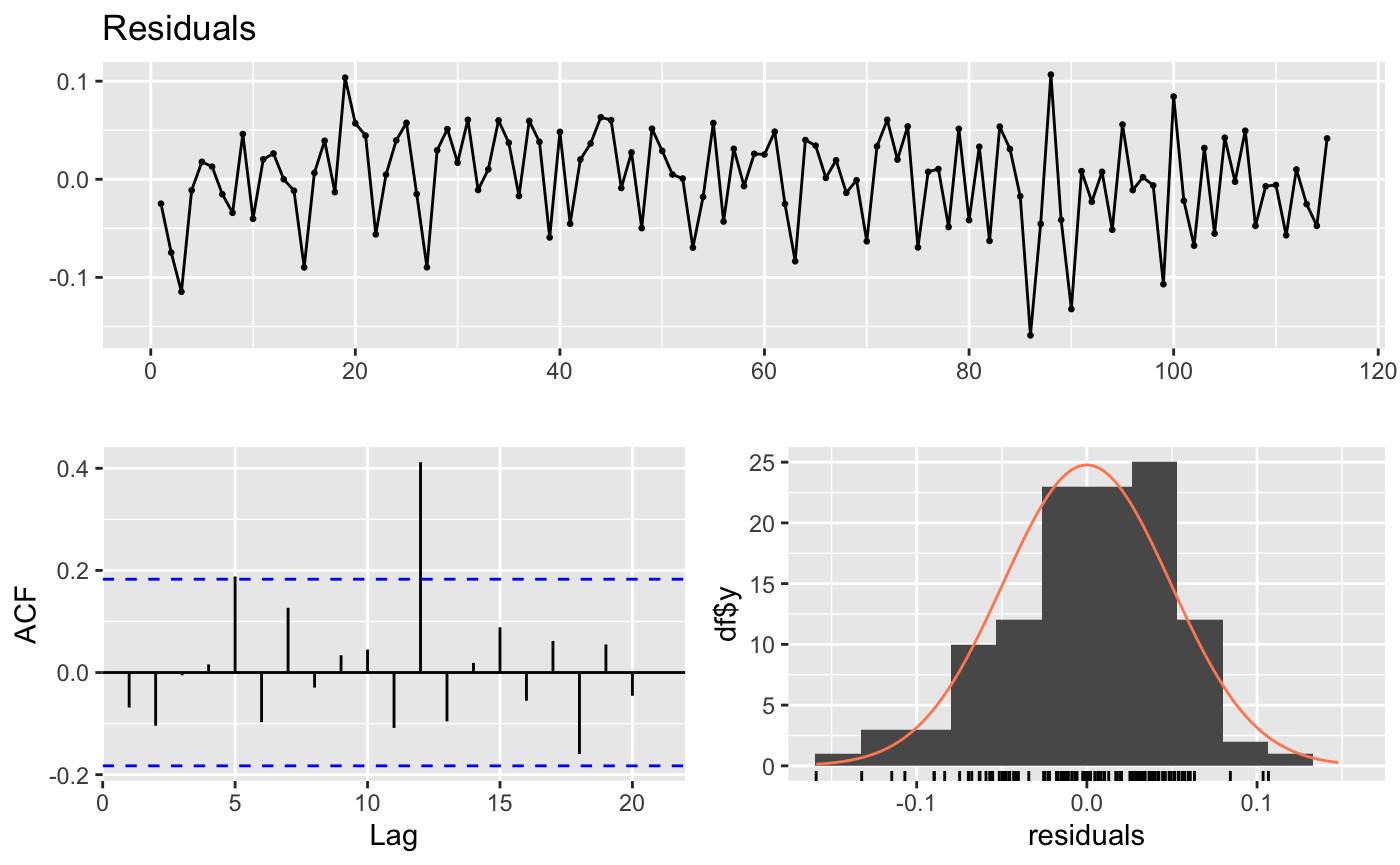
\includegraphics[width=4.2in]{var2_residuals.png}
\end{figure}
\end{frame}

\begin{frame}
\frametitle{VAR(5) Model CCF of Residuals}
\begin{figure}
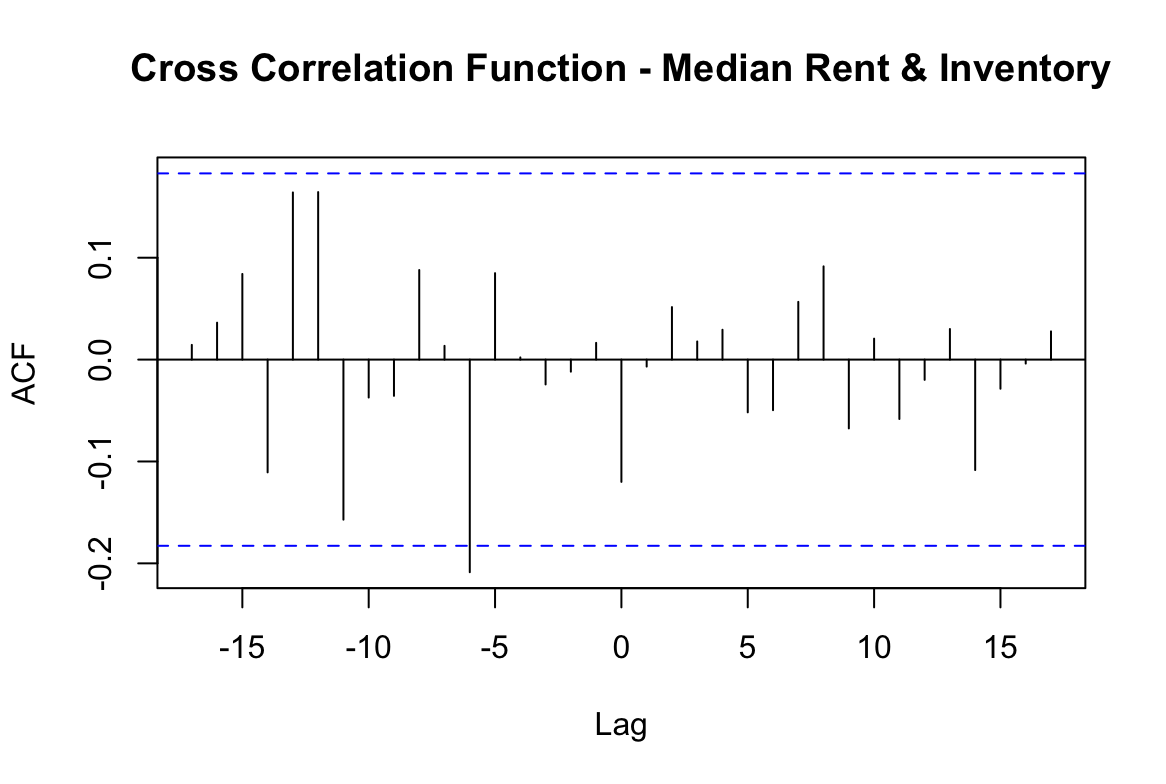
\includegraphics[width=4.2in]{var_ccf_residuals.png}
\end{figure}
\end{frame}

\end{document}